\documentclass{beamer}



\mode<presentation> %
{
  % \usetheme{Warsaw}
  % or ...
%\usetheme{Madrid}%https://www.overleaf.com/learn/latex/Beamer#Reference_guide
  % \usetheme{AnnArbor}
  % \usetheme{PaloAlto}
%   \usetheme{Darmstadt}
  \usetheme{EastLansing}
%   \usecolortheme{rose}


%   \usecolortheme{wolverine}

  \setbeamercovered{transparent}
  % or whatever (possibly just delete it)
}

\usepackage{array}
\usepackage{tabularx} 
%\usepackage{multirow}
%\usepackage{longtable}
%\usepackage{subfigure}not found
%\usepackage{lipsum}
%\usepackage[demo]{graphicx}
\usepackage{graphicx}
\usepackage{graphicx,subcaption}
\usepackage{caption}
\usepackage{subcaption}
\usepackage{xcolor}
% \usepackage{ulem}
\usepackage{soul}
%\usepackage{grffile}

% \graphicspath{ {/publicfs/cms/user/huahuil/TauOfTTTT/2016v1/v9_NewNtuple/plots_and_results/} }

\usepackage[english]{babel}
% or whatever

\usepackage[latin1]{inputenc}
% or whatever

\usepackage{times}
\usepackage[T1]{fontenc}
% Or whatever. Note that the encoding and the font should match. If T1
% does not look nice, try deleting the line with the fontenc.


\title[huilng.hua@cern.ch] % (optional, use only with long paper titles)
{IV+CV Results for HGCal Proto A Sensors}
%\subtitle
%{Include Only If Paper Has a Subtitle}
\author[Huiling Hua] % (optional, for multiple authors)
% {Huiling Hua }
{ Pedro Almeida\and Oliwia Haluszczak\and \textbf{Huiling Hua} \and Lucie Linssen\and Filip Moortgat\and Thorben Quast\and Kourosh Sarbandi\and Sicking\and Eva Sicking\and
Chaochen Yuan\and Philipp Zehetner\and \textbf{Marta Krawczyk} }
\logo{
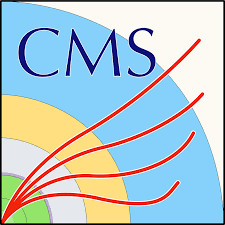
\includegraphics[width=1.0cm]{plots/CMS_Logo.png}
\includegraphics[width=1.0cm]{plots/CERN_Logo.png}
}

%\author{Huiling Hua}
%\institute{IHEP}
% \institute[IHEP] % (optional)
% {
%   \inst{1}%
%     IHEP
% }
\date[2022.02.10] % (optional, should be abbreviation of conference name)
{CMS HGCal Sensor Testing Weekly Meeting}

% - Either use conference name or its abbreviation.
% - Not really informative to the audience, more for people (including
%   yourself) who are reading the slides online
\subject{Physics Analysis}
% This is only inserted into the PDF information catalog. Can be left
% out. 

% If you have a file called "university-logo-filename.xxx", where xxx
% is a graphic format that can be processed by latex or pdflatex,
% resp., then you can add a logo as follows:
% \pgfdeclareimage[height=0.4.1cm]{university-logo}{university-logo-filename}
% \logo{\pgfuseimage{university-logo}}

% Delete this, if you do not want the table of contents to pop up at
% the beginning of each subsection:
% \AtBeginSubsection[]
% {
  % \begin{frame}<beamer>{Outline}
    % \tableofcontents[currentsection,currentsubsection]
  % \end{frame}
% }
\AtBeginSection[]
{
  \begin{frame}<beamer>{Outline}
    \tableofcontents[currentsection]
  \end{frame}
}



\begin{document}

\begin{frame}
  \titlepage
\end{frame}

% \begin{frame}{Outline}
%   \tableofcontents
  % You might wish to add the option [pausesections]
% \end{frame}
\section{Introduction}

\begin{frame}{Sensor List: High Density and Low Density}
    \begin{itemize}
        \item Compaigns: Fall2021\_PM8, EndOf2021\_PM8, LongtermIV\_ALPS\_2021, Winter2022\_ALPS
        % \item ss
    \end{itemize}    
\end{frame}

\begin{frame}{Machine Setup}
  \begin{minipage}{0.5\textwidth}
    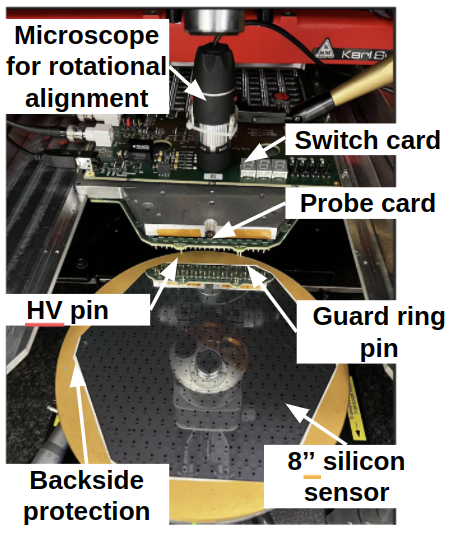
\includegraphics[scale=0.3]{plots/PM8_description.png}
    \hyperlink{https://www.sciencedirect.com/science/article/pii/S0168900219308253}{\beamergotobutton{Array System}}
  \end{minipage} \hfill
  \begin{minipage}{0.45\textwidth}
    \begin{itemize}
      \item Measurement at room temperature
      \item \text{Humidity: 40\% - 50\%}
      \item \text{Voltage up to -850V}
      \item \text{Voltage provided through the HV pin to the backside}
    \end{itemize}
  \end{minipage}
\end{frame}

\begin{frame}{Measurement Workflow}
\end{frame}
    

  

\section{IV Results}

\section{CV Results}

\section{Long Term IV}




\section*{Backup}

\begin{frame}{Backup}
	\center
	\huge
	backup
\end{frame}

\begin{frame}{List of ProtoA Sensors}
    
\end{frame}




%\begin{frame}
%\frametitle{Sample frame title}
%
%In this slide, some important text will be
%\alert{highlighted} because it's important.
%Please, don't abuse it.
%
%\begin{block}{Remark}
%Sample text
%\end{block}
%
%\begin{alertblock}{Important theorem}
%Sample text in red box
%\end{alertblock}
%
%\begin{examples}
%Sample text in green box. The title of the block is ``Examples".
%\end{examples}
%\end{frame}
%
%\begin{frame}{Make Titles Informative.}
%  You can create overlays\dots
%  \begin{itemize}
%  \item using the \texttt{pause} command:
%    \begin{itemize}
%    \item
%      First item.
%      \pause
%    \item    
%      Second item.
%    \end{itemize}
%  \item
%    using overlay specifications:
%    \begin{itemize}
%    \item<3->
%      First item.
%    \item<4->
%      Second item.
%    \end{itemize}
%  \item
%    using the general \texttt{uncover} command:
%    \begin{itemize}
%      \uncover<5->{\item
%        First item.}
%      \uncover<6->{\item
%        Second item.}
%    \end{itemize}
%  \end{itemize}
%\end{frame}
%
%
%% All of the following is optional and typically not needed. 
%\appendix
%\section<presentation>*{\appendixname}
%\subsection<presentation>*{For Further Reading}
%
%\begin{frame}[allowframebreaks]
%  \frametitle<presentation>{For Further Reading}
%    
%  \begin{thebibliography}{10}
%    
%  \beamertemplatebookbibitems
%  % Start with overview books.
%
%  \bibitem{Author1990}
%    A.~Author.
%    \newblock {\em Handbook of Everything}.
%    \newblock Some Press, 1990.
% 
%    
%  \beamertemplatearticlebibitems
%  % Followed by interesting articles. Keep the list short. 
%
%  \bibitem{Someone2000}
%    S.~Someone.
%    \newblock On this and that.
%    \newblock {\em Journal of This and That}, 2(1):50--100,
%    2000.
%  \end{thebibliography}
%\end{frame}

\end{document}


